\chapter{Prestaciones Exigidas a las Estructuras}
\section{Introducción}
A las estructuras se les exigen prestaciones de muy distintas índole como p.e. las relativas a la seguridad estructural y otras relacionadas con la funcionalidad o la estética. El grado de cumplimiento de cada una de ellas permite y facilita la comparación de diferentes soluciones para la misma estructura.

Es evidente que la mejor solución o el diseño óptimo depende de la ponderación de las diferentes prestaciones. El marco normativo prescribe procedimientos y métodos de cálculo y además establece valores límite para garantizar el cumplimiento de unos requisitos mínimos. Por tanto existen múltiples diseños / soluciones aceptables desde el punto de vista normativo.

La hipótesis de carga tienen un impacto importante en el precio final de la obra y, aunque no debería ser así, en algunos países se ajustan dichas hipótesis a la baja reduciendo de esa forma el margen de seguridad de las estructuras ante acciones sísmicas para reducir los costes.

\section{Palabras clave y principios generales}
En función del contexto en el que se usan la palabras su sentido puede variar un poco y en lo que se refiere al proyecto estructural conviene saber el significado de los siguientes conceptos o características.

% Añadir las cosas del documento PDF que está en la Moodle

\begin{itemize}
    \item Proporcionalidad
    \item Robustez del diseñoRedundancia estructural
    \item Facilidad de construcción
    \item Facilidad de inspección
    \item Definición y contenido de una normativo
    \item Diferencia entre una norma y un reglamento
    \item Proyecto básico o proyecto de ejecución
\end{itemize}

\section{Marco normativo para el proyecto}  
En la actualidad se están utilizando normas elaboradas en España conjuntamente con los Eurocódigos (UNE-EN-199X). El 10 de noviembre de 2021 entró en vigos el Código Estructural que facilita la transición del conjunto de normas nacionales a las europeas.

\begin{figure}[H]
    \centering
    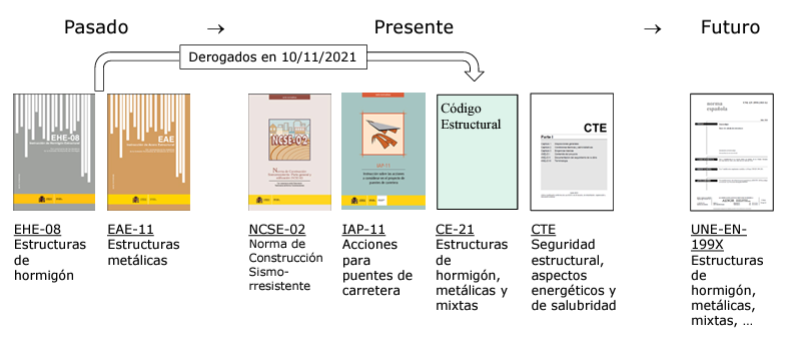
\includegraphics[width = 0.5 \textwidth]{Imagenes/Marco normativo para el proyecto.png}
    %\caption{Marco normativo para el proyecto.}
\end{figure}

\subsection{Eurocódigos}
Los 10 Eurocódigos están redactados en 58 partes. En total son miles de páginas. Se revisan y actualizan periódicamente.

\begin{table}[H]
    \centering
    \begin{tabular}{| p{8cm} |}
        \hline
        EN 1990: Eurocódigos. Bases de cálculo de estructuras. \\
        \hline
        EN 1991: Eurocódigo 1: Acciones en estructuras. \\
        \hline
        EN 1992: Eurocódigo 2: Proyecto de estructuras de hormigón. \\
        EN 1993: Eurocódigo 3: Proyecto de estructuras de acero. \\
        EN 1994: Eurocógido 4: Proyecto de estructuras mixtas de acero y hormigón. \\
        EN 1995: Eurocódigo 5: Proyecto de estructuras de madera. \\
        EN 1996: Eurocódigo 6: Proyecto de estructuras de fábrica. \\
        EN 1999: Eurocódigo 9: Proyecto de estructuras de aluminio. \\
        \hline
        EN 1997: Eurocódigo 7: Proyecto geotécnico. \\
        EN 1998: Eurocódigo 8: Proyecto de estructuras sismorresistentes. \\
        \hline
    \end{tabular}
\end{table}

Cada país miembro de la UE redacta los anejos nacionales en loa que se fijan algunos prámetros que hacen falata para la aplicación de los métodos de cálculo descritos en los Eurocódicos, p.e. factores parciales de seguridad

\subsubsection{Algunas áreas de actuación}

Edificios, construcciones representativas, naves industriales e instalaciones Industriales como p.e.
\begin{itemize}
    \item Depósitos y recipientes a presión (p.e. gas natural)
    \item Edificios de contención en centrales nucleares
    \item Líneas de transporte de energía eléctrica
    \item Grandes antenas parabólicas, colectores fotovoltaicos, etc.
\end{itemize}

Con menos frecuencia el ingeniero industrial está involucrado en la parte de la obra civil o túneles pero sí en el diseño instalaciones (eléctricas, ventilación, señalización, monitorización de parámetros de interés p.e. de un puente en zona sísmica, Internet of Things - IoT, gemelo digital).

\section{Prestaciones en servicio}

El objetivo de la comprobación de los estados límite de servicio consiste en garantizar un comportamiento adecuado de la estructura ante combinaciones de carga frecuentes.

\begin{itemize}
    \item modos de fallo no se refieren a la integridad estructural
    \item garantizar confort de los usuarios y correcto funcionamiento del Edificios
    \item aptitud al servicio teniendo en cuenta el uso previsto del Edificios
\end{itemize}

El CTE contempla los siguiente estados límite de servicio:
\begin{itemize}
    \item deformaciones: flechas, asientos o desplomes
    \item vibraciones: falta de confort de usuarios, funcionalidad reducida de la obra
    \item daños o el deterioro que pueden afectar desfavorablemente a la apariencia, a la durabilidad o a la funcionalidad de la obra
\end{itemize}

\section{Prestaciones en seguridad}

El objetivo de los estados límite último consiste en garantizar la seguridad de los usuarios y de aquellas personas que se encuentran en espacios públicos cercanos. Los modos de fallo se refieren a la integridad estructural de la estructura así que superar un estado límite último constituye un riesgo para las personas, ya sea porque produce una puesta fuera de servicio de la estructura o el colapso total o parcial de la misma.

El CTE contempla los siguientes estados límite último:
\begin{itemize}
    \item pérdida del equilibrio del edificio, o de una parte estructuralmente independiente, considerado como un cuerpo rígido
    \item fallo por deformación excesiva, transformación de la estructura o de parte de ella en un mecanismo, rotura de sus elementos estructurales (incluidos los apoyos y la cimentación) o de sus uniones
    \item inestabilidad de elementos estructurales incluyendo los originados por efectos dependientes del tiempo (corrosión, fatiga)
\end{itemize}

\subsection{Definiciones de fallo}
Basado en la capacidad del material de experimentar deformación plástica se distingue entre 
\begin{itemize}
    \item Fallo dúctil: Antes de la rotura se producen deformaciones muy importantes que llaman la atención incluso a personas no expertas - capacidad de aviso
    \item Fallo frágil: antes de la rotura se producen pocas o nulas deformaciones plásticas - capacidad de aviso muy pequeña o nula
\end{itemize}
Por la importancia de la capacidad de aviso las normas hacen hincapié en evitar la rotura frágil de elementos estructurales.

Basado en la extensión del fallo se distingue entre:
\begin{itemize}
    \item Fallo parcial: El fallo se limita a uno o pocos elementos estructurales y sólo afecta a una parte de la estructura. Después se produce una redistribución de fuerzas.
    \item Fallo global: El fallo y la posterior redistribución de fuerzas provoca un mecanismo que afecta a toda la estructura.
\end{itemize}

Para evitar fallos globales hay que impedir la propagación del fallo inicial. Requisito indispensable para ello es normalmente un cierto grados de redundancia del sistema estructural es decir existen caminos de transmisión alternativos para llevar las cargas muertas y vivas a la cimentación.

\section{Comprobación de las prestaciones mediante cálculo}

En el cálculo estructural se han empleado durante las últimas décadas diferentes tipos de comprobación entre los que se encuentran comprobaciones
\begin{itemize}
    \item determinista: los valores de las diferentes acciones y resistencias son perfectamente conocidos
    \item probabilista: los valores de las diferentes acciones y resistencias siguen funciones de distribución; como resultado se obtiene la probabilidad de fallo
    \item semi-probabilistas: se caracterizan las diferentes acciones y resistencias con valores nominales que se combinan con coeficientes parciales de seguridad para determinar
\end{itemize}
Se suelen utilizar métodos probabilistas para calibrar los coeficientes parciales de seguridad de los métodos semi-probabilistas.

\subsubsection{Evolución de los conceptos de seguridad}
Método clásico o de la tensión admisible.
Se distinguen entre diferentes estados de carga.
\begin{itemize}
    \item Estado de carga I: Cargas permanentes, sobrecargas de explotación, sobrecargas de nieve, efectos producidos por asientos o posibles movimientos de apoyos y sobrecargas de ejecución.
    \[ \sigma \leq \sigma_{adm} = \frac{\sigma_y}{1.5} \quad \sigma_y \textup{ tensión de fluencia } \]
    \item Estado de carga II: Además de las anteriores, acciónd el viento, efectos térmicos, efectos del frenado y empuje lateral de los puentes grúa y efectos sísmicos.
    \[ \sigma \leq \sigma_{adm} = \frac{\sigma_y}{1.33} \]
\end{itemize}

Métodos de los estados límites
Se definen estados límite, las situaciones a comprobar así como factores parciales de seguridad para mayorar las cargas y minorar las resistencias

\[ S(\gamma_{Si} F_{ki}) \leq R(f_{kj}/ \gamma_ {Rj}) \]

\subsection{Fiabilidad estructural}
La fiabilidad de une estructura es la capacidad de cumplir los objetivos por los que ha sido diseñada durante un periodo de referencia.

La fiabilidad $R$ de un sisrema se define como sigue:
\[R = 1 - P_f\]

Las diferentes formas de fallo de uns estructura se llaman modos de fallo. Primero se calcula la probabilidad de fallo de cada uno de ellos y a continuación la de la estructura (fiabilidad de sistemas).

Para el cálculo de la probabilidad de fallo están disponibles
\begin{itemize}
    \item Métodos de nivel 1: valores caracrerísticos + factores parciales de ``seguridad'' % no tenemos como resultado una probabilidad de fallo
    \item Métodos de nivel 2: funciones de distribución de las variables de carga y resistencia $ \rightarrow P_f$
    \item Métodos de nivel 3: funciones de distribución conjuntas y superficies de fallo exactas $\rightarrow P_f$
\end{itemize}

\subsubsection{Caso fundamental de fiabilidad}
En algunas situaciones puede describirese la fiabilidad de un elemento d euna estructura con sólo dos variables aleatorias independientes, una carga S y otra de resistencia R. En este caso el criterio de fallo queda definido como sigue:
\[R - S < 0\]
La probabilidad de que la carga este en el intervalo entre $x - dx/2$ y $x + dx/2$ es $f_s(x)dx$.

% si integramos una función de densidad obtenemos una función de distribución

\begin{figure}[h]
    \centering
    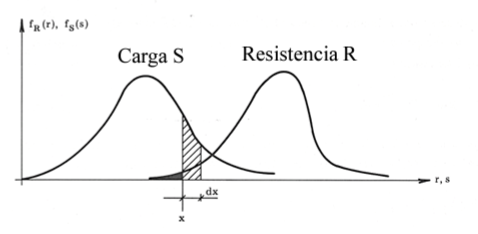
\includegraphics[width = 0.5 \textwidth]{Imagenes/Fiabilidad estructural - Funciones de densidad.png}
    \caption{Funciones de densidad.}
\end{figure}

La probabilidad de que la resistencia sea menor que la carga es $F_R(x)$ y por tanto la probabilidad de fallo es $F_R(x)f_Sdx$.

La probabilidad de fallo total se obtiene integrando sobre $x$.
\[ P_f = \int_{- \infty}^\infty{F_R(x) f_s (x) dx} \]

Siendo:
\begin{itemize}
    \item $f_R$: función de densidad de la variable $R$
    \item $F_R$: función de distribución de la variable $R$
\end{itemize}

\subsubsection{Índices de fiabilidad}
La evaluación de la integral para el cálculo de la probabilidad de fallo suele ser muy complicada y soluciones analíticas sólo existen para casos especiales como el siguiente:
\begin{itemize}
    \item R y S son independientes y siguen una distribución normal ($N(\mu_R, \sigma_R)$ y $N(\mu_S, \sigma_S)$)
    \item se define M = R - S como margan de seguridad que sigue $N(\mu_M, \sigma_M)$ con $\mu_M = \mu_R - \mu_S$ y $\sigma_M^2 = \sigma_R^2 + \sigma_S^2$
    \item $P_f$ se obtiene como la función de distribución normal estándar $\phi$ 
    \[ P_f = P (R - S \leq 0) = P(M \leq 0) = \phi \left( \frac{0 - \mu_M}{\sigma_M} \right) = \]
    \[ = \phi \left( \frac{\mu_S - \mu_R}{\sqrt{\sigma_R^2 + \sigma_S^2}} \right) = \phi(-\beta) \rightarrow \beta = -\phi^{-1}(P_f)\]
\end{itemize}

El índice de fiabilidad $\beta$ de Cornell está definido como cociente entre los valores entre el valor esperado del margen de seguridad y su desviación típica.
\[\beta = \frac{\mu_M}{\sigma_M} \rightarrow \mu_M = \beta \sigma_M\]

\begin{figure}[h]
    \centering
    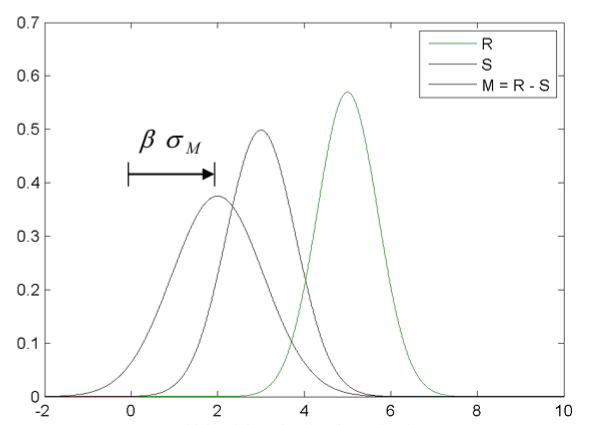
\includegraphics[width = 0.5 \textwidth]{Imagenes/Fiabilidad estructural - Valor del parametro de contraste.png}
    \caption{Valor del parámetro de contraste.}
\end{figure}

% si nos proporcionan la distribuciones de la carga de resistencia tenemos que saber calcular el valor medio y la desviación típica y nosotros tenemos que saber calcular el índice de fiabilidad 

El índice de fiabilidad de Cornell tiene la desvestaja de depender de la función que se utiliza para desscribir la superficie de fallo. Teniendo en cuenta que existen infinitas funciones para describir la misma superficie de fallo se trata de un punto débil importante.

\[ M_1 = R - S \quad M_2 = 1 - \frac{S}{R} \quad P_{f, M_1} = P_{f, M_2} \quad \beta_{M_1} \neq \beta_{M_2} \]

Hasofer y Lind propusieron una definición alternativa, que no tiene este defecto, utilizando variables normalizadas

\[ \bar{R} = \frac{R - \mu_R}{\sigma_R} \quad \bar{S} = \frac{S - \mu_S}{\sigma_S} \quad \bar{M} = f(\bar{R}, \bar{S})\]

y definiendo el índice de fiabilida $\beta$ como distancia mínima entre el origen del espacio de coordenadas normalizdas y la superficie de fallo. Esta definición tiene la ventaja de establecer reglas claras para el caso de una función de fallo no-lineal que se aproxima por un hiperplano.

\begin{figure}[H]
    \centering
    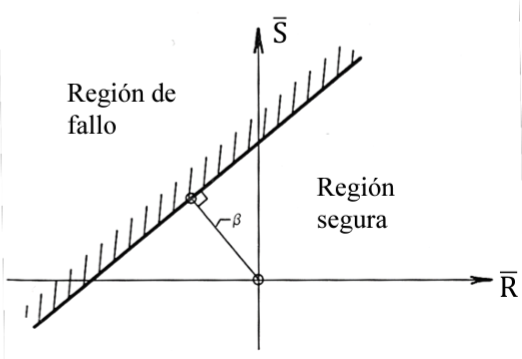
\includegraphics[width = 0.5 \textwidth]{Imagenes/Fiabilidad estructural - Region de fallo .png}
\end{figure}

% beta es la didstancia desde el origen hasta la superficie de fallo. El punto más cercano se llama punto de proyecto

\subsubsection{Índice de fiabilidad requerido según el CTE}
El documento básico SE del CTE contiene la siguiente tabla que resume los valores mínimos del índice de fiabilidad.

\begin{figure}[H]
    \centering
    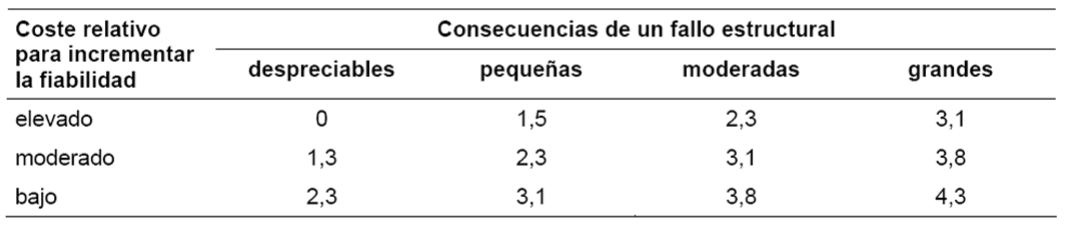
\includegraphics[width = 0.5 \textwidth]{Imagenes/Fiabilidad estructural - Indice de fiabilidad requerido segun el CTE.png}
    \caption{Valores nominales, referidos a todo el periodo de servicio, para el índice de fiabilidad requerido.}
\end{figure}

Relación entre el índice de fiabilidad $\beta$ y la probabilidad de fallo $P_f$.

\begin{table}[H]
    \centering
    \begin{tabular}{|c|c|c|c|c|c|c|c|}
        \hline
        $\beta$ & $1.3$ & $2.3$ & $3.1$ & $3.7$ & $4.3$ & $4.8$ & $5.2$ \\
        \hline
        $P_f$ & $10^{-1}$ & $10^{-2}$ & $10^{-3}$ & $10^{-4}$ & $10^{-5}$ & $10^{-6}$ & $10^{-7}$ \\
        \hline
    \end{tabular}
\end{table}

% en el examen nos pueden preguntar por indices de fiabilidad de la CTE y decir si son altos, bajos o medios...(?)

\subsubsection{Valores orientativos para la vida útil de diferentes estructuras}
La siguiente tabla se ha extraído del anejo 18 del Código Estructural.

\begin{figure}[H]
    \centering
    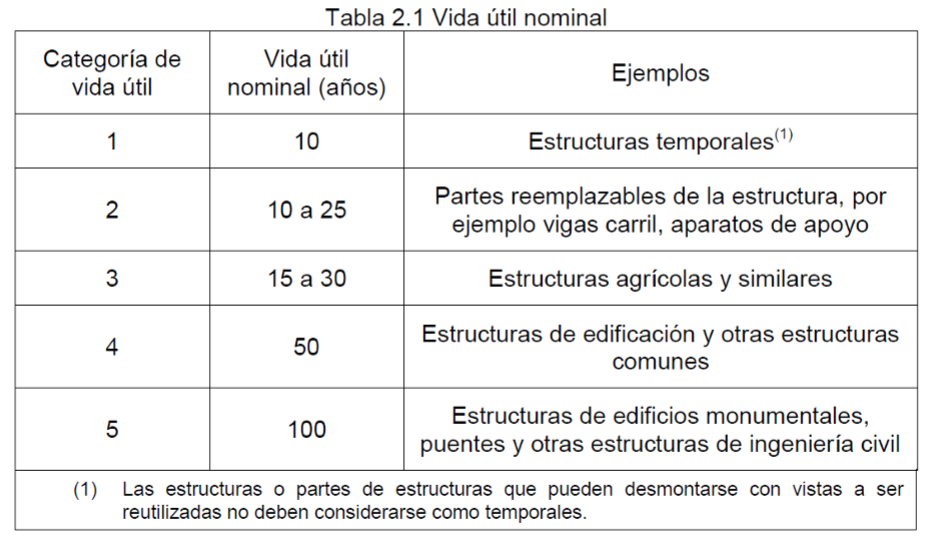
\includegraphics[width = 0.5 \textwidth]{Imagenes/Fiabilidad estructural - Vida util nominal.png}
\end{figure}

\subsubsection{Resumen métodos probabilistas}
\begin{itemize}
    \item Métodos de nivel I, II y III.  Mayor nivel, más precisión a cambio de más información (¿disponibilidad de esa información)
    \item Variables de carga y resistencia con sus distribuciones
    \item Margan de seguridad y problema fundamentalde la fiabilidad
    \item Índice de fiabilidad de Cornell: Cociente entre le valor esperado del margen de seguridad y su desviación típica. ¡Generalmente depende de la expresión que define el margen de seguridad!
    \item Índice de fiabilidad de Hasofer Lind: Distancia mínima entre el origen y la superficie de fallo en el sistema de coordenadas normalizadas
    \item El punto de proyecto puede utilizarse para calibrar los factores parciales de seguridad de métodos de nivel I
    \item Como consecuencia del avance de la tecnología informática se recurre cada vez más a métodos de simulación del tipo Monte Carlo para la evaluación de la integral para calcular la probabilidad de fallo
\end{itemize}

\subsection{Implementación a nivel normativo}
El método de los factores parciales pertenece a los métodos semi-probabilistas. A estos métodos el CTE les denomina Métodos Probabilistas Implicitos. Fijando la probabilidad de fallo admisible a través del índice de fiabilidad $\beta$ y admitiendo que
\begin{itemize}
    \item las acciones actúan en combinaciones predefinidas
    \item la distribución de cada una de tales combinaciones responde a un tipo concreto 
    \item las relaciones entre acciones y solicitaciones son conocidad
\end{itemize}
entonces es posible obtener el valor de los coeficientes $\gamma_S$ y $\gamma_R$ tales que:
\[ S(\gamma_{Si} F_{ki}) < R(f_{ki} / \gamma_{Rj}) \]

La administración regula:
\begin{itemize}
    \item El nivel de seguridad
    \begin{itemize}
        \item Valor del índice de fiabilidad $\beta$
        \item Valores de los factores parciales $\gamma_R$ y $\gamma_S$
        \item Valores de las acciones $F$
        \item Valores de las resistencias $f$
    \end{itemize}
    \item La definición de fallo
    \begin{itemize}
        \item Estado Límite Último (ELU)
        \item Estado Límite de Servicio (ELS)
    \end{itemize}
    \item Las situaciones a comprobar
    \begin{itemize}
        \item Permanente
        \item Transitoria
        \item Sísmica
        \item Accidental
    \end{itemize}
\end{itemize}

Factores parciales para las acciones

\begin{figure}[H]
    \centering
    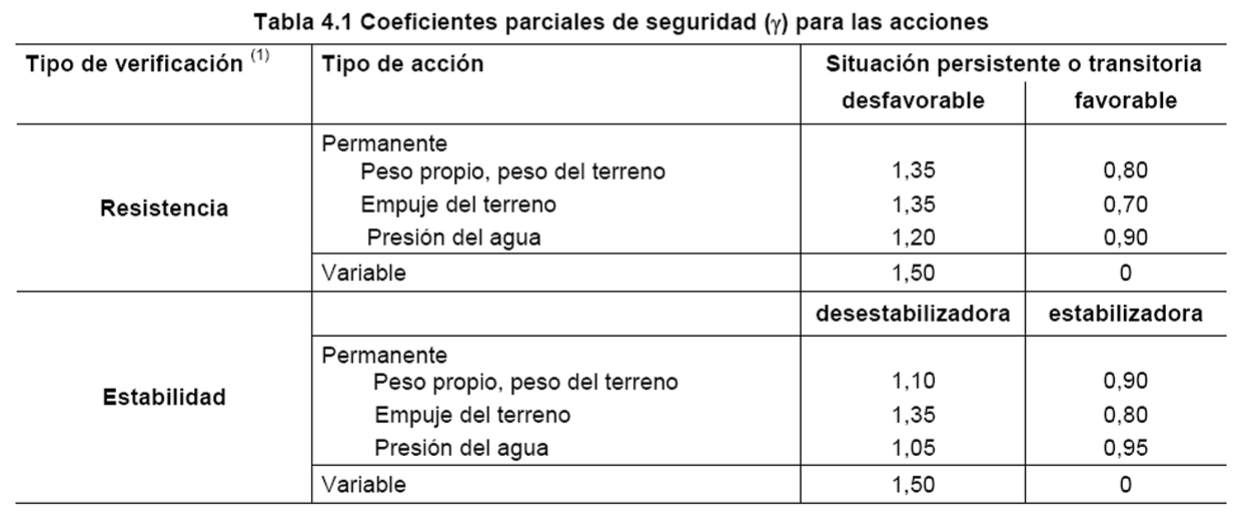
\includegraphics[width = 0.5  \textwidth]{Imagenes/Implementacion a nivel normativo - Factores parciales para las acciones.png}
\end{figure}

Factores parciales para la resistencia

\begin{figure}[H]
    \centering
    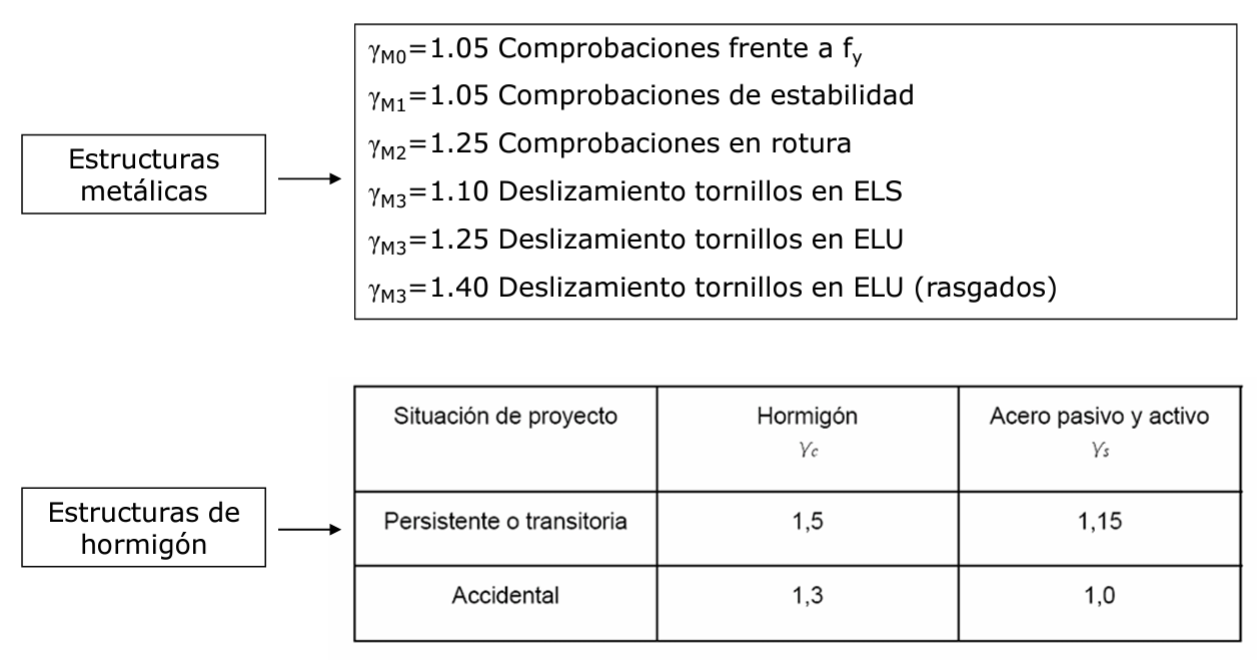
\includegraphics[width = 0.5  \textwidth]{Imagenes/Implementacion a nivel normativo - Factores parciales para la resistencia.png}
\end{figure}

En general se distingue entre:
\begin{itemize}
    \item acción directa: Fuerza aplicada sobre el Edificios
    \item acción indirecta: Deformación impuesta o aceleración causada por cambios de temperatura, variaciones de humedad, asientos diferenciales o sismos
\end{itemize}

Clasificación de acciones:
\begin{itemize}
    \item Variación en el tiempo:
    \begin{itemize}
        \item Permanentes (G): de valor constante (peso propio), de valor no constante (pretensado, acciones del terreno)
        \item Variables (Q): sobrecarga de uso (efectos derivados del uso normal), viento, nieve
        \item Accidentales (A): impactos, acción sísmica
    \end{itemize}
    \item Variación en el espacio:
    \begin{itemize}
        \item Fijas: Peso propio, elementos funcionales
        \item Libres: Sobrecargas de uso, cargas de tráfico, nieve
    \end{itemize}
\end{itemize}

\begin{figure}[H]
    \centering
    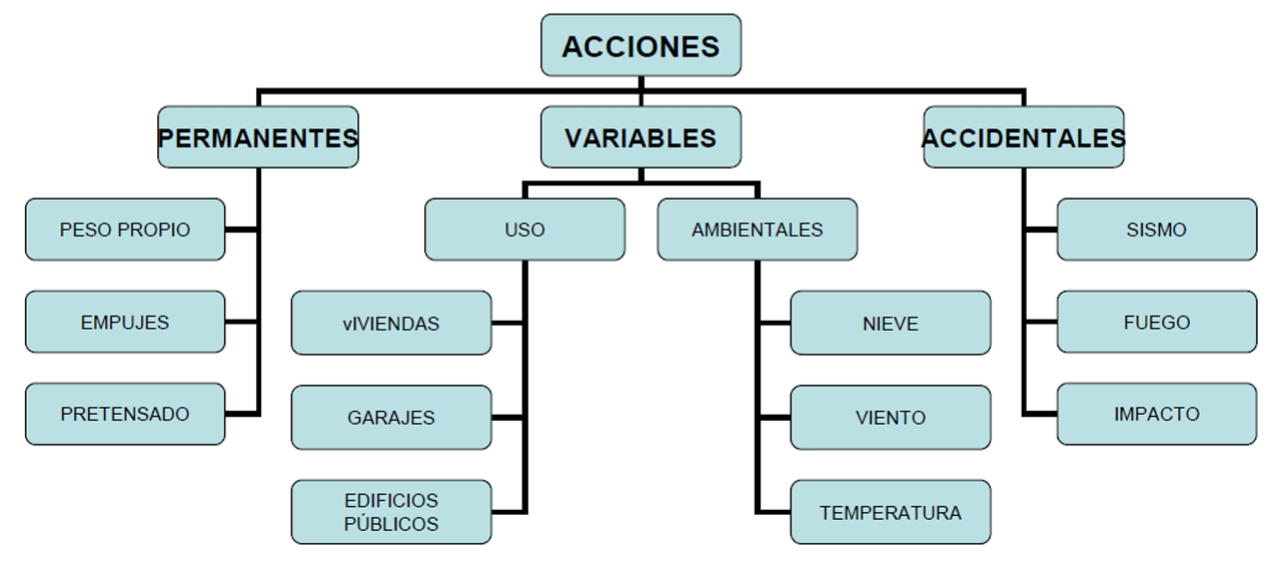
\includegraphics[width = 0.5 \textwidth]{Imagenes/Implementacion a nivel normativo - Clasificacion de acciones.png}
\end{figure}

Para la comprobación de los estados límite se modifica el valor característico de la acción en función de la situación de comprobación.

Conviene distinguir entre:
\begin{itemize}
    \item Valor característico: valor de una acción, $F_k$, que se define, según el caso, por su valor medio, por un fractil superior o inferior, o por un valor nominal.
    \item Valor representativo: producto del valor característico $F_k$ y el coeficiente de simultaneidad $\psi_i$. Se utilizan los coeficientes de simultaneidad para no generar hipótesis de cálculo muy improbables o físicamente imposibles como p.e. que la carga de nieve y la de viento alcancen simultáneamente sus valores máximos.
    \item Valor de cálculo: producto del valor característico o representativo por el coeficiente parcial de seguridad $\gamma_f$. El coeficiente $\gamma_f$ puede ser mayor o menor que la unidad en función de si la carga actúa de manera desfavorable o no.
\end{itemize}

Formato de las comprobaciones para la ELU:

Estabilidad: $E_{d, dst} \leq E_{d, stb}$
siendo:
\begin{itemize}
    \item $E_{d, dst}$ valor de cálculo del efecto de las acciones desestabilizadoras
    \item $E_{d, stb}$ valor de cálculo del efecto de las acciones estabilizadoras
\end{itemize}

Resistencia: $E_d \leq R_d$
siendo:
\begin{itemize}
    \item $E_d$ valor de cálculo del efecto de las acciones
    \item $R_d$ valor de cálculo de la resistencia correspondiente
\end{itemize}

\begin{figure}[H]
    \centering
    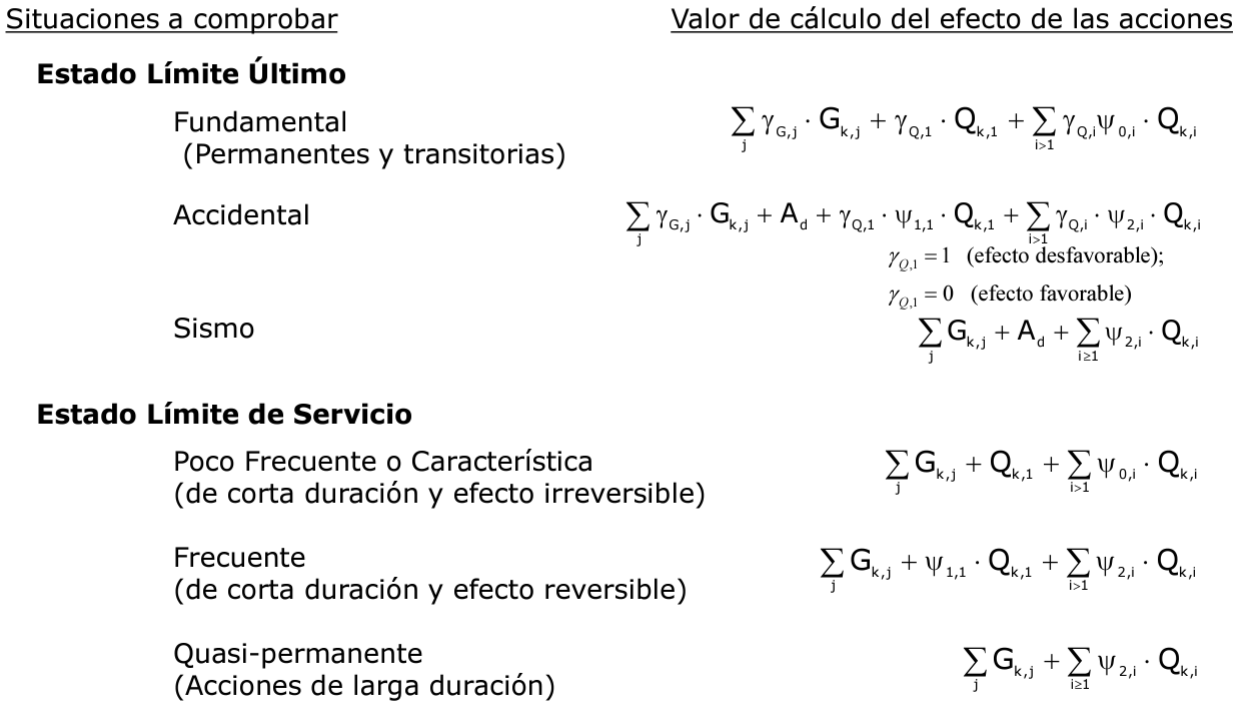
\includegraphics[width = 0.5 \textwidth]{Imagenes/Implementacion a nivel normativo - Situaciones a comprobar.png}
\end{figure}

\subsubsection{Organización de las comprobaciones}
En general la comprobación ante cada estado límite se realiza en dos fases:
\begin{itemize}
    \item Análisis: Determinación de los esfuerzos y desplazamientos globales. Por ejemplo utilizando un modelo de elemntos finitos se obtienen los desplazamientos nodales y las reacciones. A partir de los desplazamientos se calculan los esfuerzos y tensiones.
    \item Comprobación: Se calculan las capacidades resistentes de las secciones y elementos estructurales y se comparan los valores resultantes con las solicitaciones.
\end{itemize}

Tanto el análisis como la comprobación peude hacerse en régimen elástico o plástico. Normalmente se emplean modelos elásticos y lineales en las comprobaciones frente a estados límite de servicio.